\subsection{Simulated 2023 storm surge results}
Based on the results of the simulated 2023 storm surge, a number of factors can be discussed. The choice to start all simulations at 100 centimetres is debatable. It was done in order to minimise the processing duration, since a vast majority of area below 100 centimetres are out by the coastline and there is therefore not that much difference between starting the simulation at 100 or 0.1 centimetres. It would also have added at least 50\% more processing duration for each site without contributing to the overall final result.\\
Similarly, the simulations were performed with an increment value of one centimetre. This was the lowest increment value that was realistic to the simulations at. However it has contributed to a longer processing duration, and had the areas been larger, it would have added significantly more to total processing runtime.\\

The results from the Inundation Model to simulate the extent of the 2023-storm surge event have been reasonable. Two of the sites: Gedser Havn and Hesnæs, both have had simulated results that closely reflects the observed data (figure \ref{Figur: Målt & simuleret Gedser} and \ref{Figur: Målt & simuleret Hesnæs}). Both of these two areas however had a smaller inundated area than the observed data. This could be an indication that the model might be underestimating the extent of a storm surge. If this study included more sites, it might have been possible to better assess whether this is true or not. Since there are only two results that are not affected by other reasons, it is not possible to confirm this.\\

Aabenraa and Præstø, on the other hand, have had a larger and a smaller area flooded respectively in the Inundation Model's results than what happend during the storm surge in 2023 due to several external factors that occurred during the event back in October of 2023.
\begin{figure}[H]
	\centering
	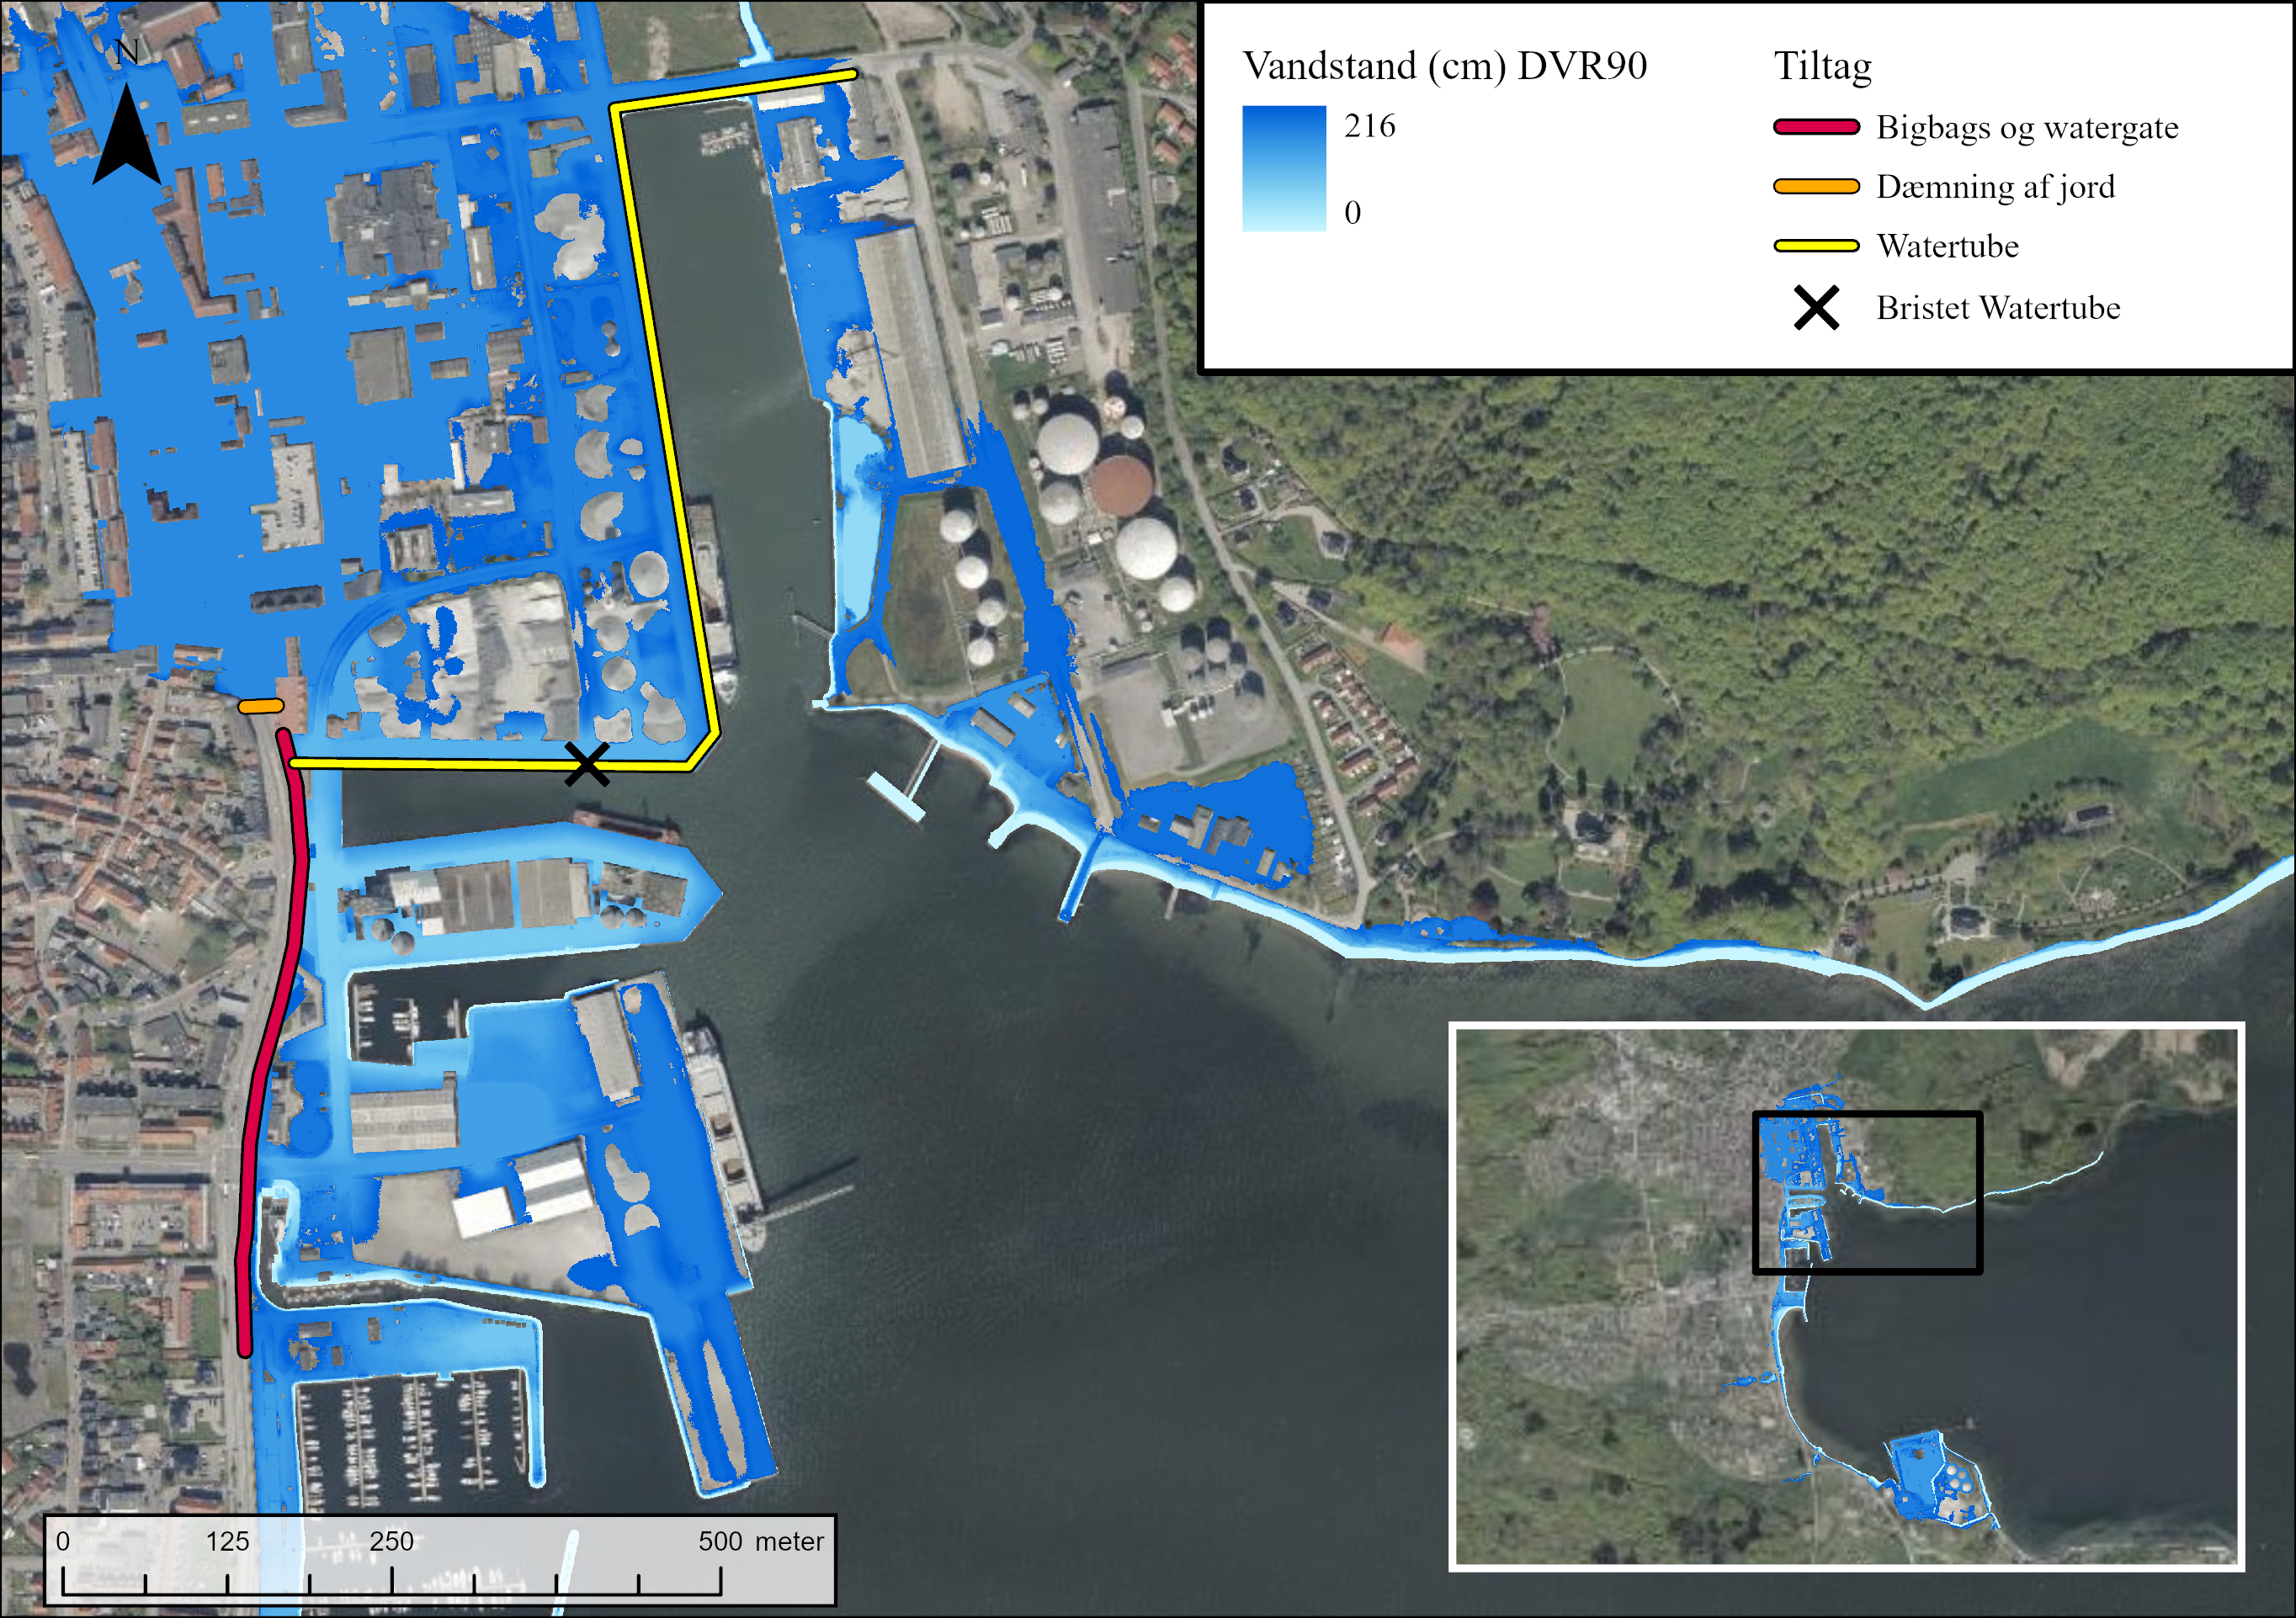
\includegraphics[width=0.8\linewidth]{images/diskussion/beredskabstiltag.jpg}
	\caption{Kort over beredskabstiltag foretaget i løbet af den 20. oktober 2023 i Aabenraa og den observeret oversvømmelse. Dæmningen af jord blev etableret efter watertuben bristede. Kilde: Aabenraa Kommune}
	\label{Figur: Beredskabstiltag}
\end{figure}
For Aabenraa, the main difference between observed and simulated results is caused by a set of emergency measures implemented along the harbour during the storm surge on October 20th, 2023. (Figure \ref{Figur: Beredskabstiltag}). This included an approximately 1 kilometre long watertube and barricades of BigBag sandbags along the harbour quay and the main road. The black cross in figure \ref{Figur: Beredskabstiltag} indicates where the watertube burst due to the water pressure. Despite this rupture, the local emergency services, Brand og Redning Sønderjylland, managed to establish a barricade with bags of soil that prevented the water from flowing south and further into Aabenraa city centre and thus the area behind which was flooded in the result from the Inundation Model shown in figure \ref{Subfig: Model Aabenraa}.\\

In addition, there have been two small areas in the observed data where the model has not indicated a flood. The two areas are both smaller watercourses between Aabenraa City and Ensted Industrial Port (figure \ref{Figur: Tilpasnings fejl}).
\begin{figure}[H]
	\centering
	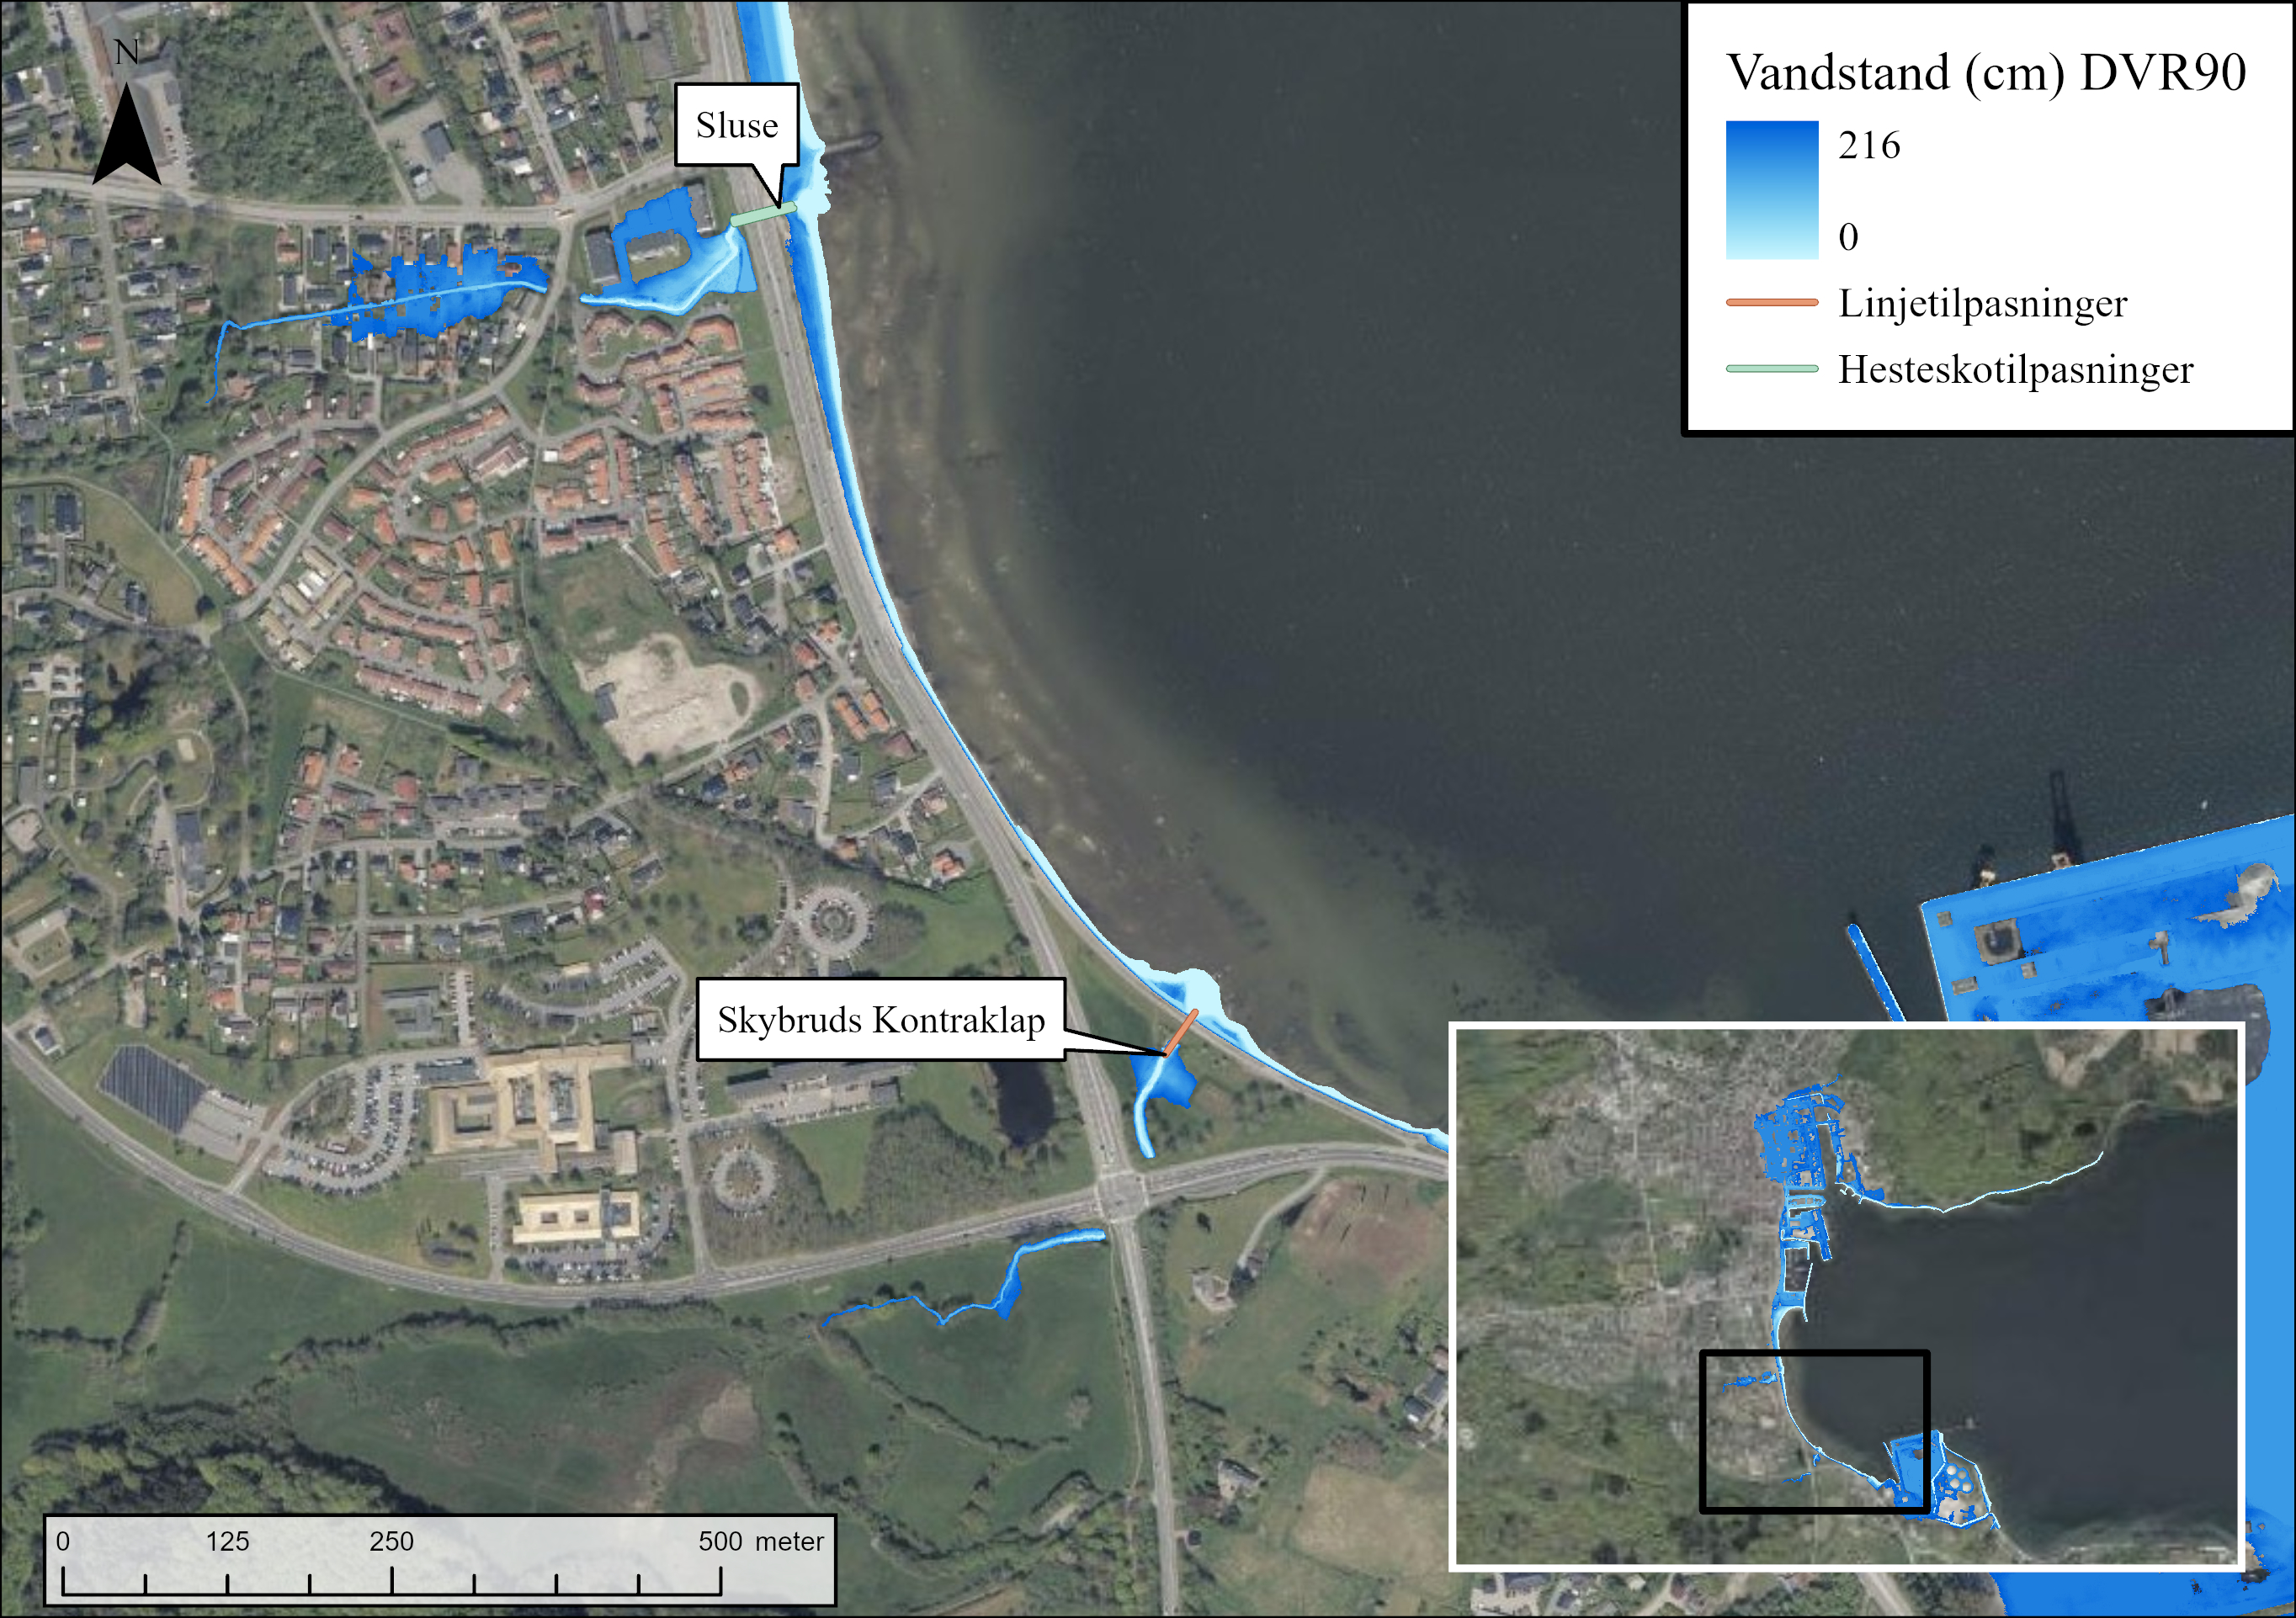
\includegraphics[width=0.8\linewidth]{images/diskussion/tilpasnings_error.jpg}
	\caption{Kort over to hydrologiske tilpasninger der ved fejl ikke er implementeret korrekt i kortet modtaget fra Aabenraa Kommune.}
	\label{Figur: Tilpasnings fejl}
\end{figure}
Both watercourses have an outlet to the fjord. The northernmost adaptation is a horseshoe adaptation with a classification as a high water-sluice lock. This would have been closed during the storm surge, and there is no sources that indicate that this lock collapsed or was open during the storm surge. The other adaptation further south is a no-return valve used to carry water from the land out into the sea during extreme rainfall. Both objects are current and active from 2015, so the assumption of changed usage must be rejected. It is therefore likely that Aabenraa municipality has mistakenly forgotten to include the two hydrological adaptations in the dataset, as other similar adaptations have been correctly implemented or that the water has penetrated through in another fashion.\\

In Præstø, the primary difference between simulated and observed data has been caused by the collapse of the sluice gate at the mouth of Tubæk Å. This incident occurred around 15:00 UTC October 20th, 2023. This incident caused most of the Tubæk Å valley area and surrounding parts to be flooded. This has not been captured by the Inundation Model as it is an unforeseen event. It is therefore debatable whether the extents would be similar if the sluice gate had not collapsed.\\

\subsection{Errors regarding calculating the projected storm surge extent.}
The simulations of future storm surges in the form of 100-year events and the projection of the 2023-storm surge for two SSP scenarios have been reasonable. Since the result of the 100-year events are directly from DMI, the result here is as expected. The calculation to project the 2023 storm surge, however, has been more debatable. The projection was based on the median value of the IPCC's projections for 2030 and DMI's expected water level at the end of the 21st century. The mere fact that the calculation is based on a median implies that there is an uncertainty interval with a potentially higher and lower water level. This interval has not been taken into account and an uncertainty interval for the mean water level in 2023 has therefore not been calculated. Another source of error in this calculation is that it assumes sea level rise since 1995 has been linear. Here it is worth noting that the degree of this error cannot be immediately documented, and \cite{danish_meteorological_institute_dmi_2024} also assumes the same linear development. It is therefore important to emphasise that this calculation thus assumes that the increase is linear and therefore does not necessarily reflect observed data and is maybe not applicable everywhere in the world. Regardless of this assumption, the projection of the storm surge has resulted in reasonable values that are not unrealistic for the location and SSP-scenario they were calculated for.\\

\subsection{Inclusion of buildings in the DHyM}
One of the more prominent methodological considerations that was taken early in the workflow was to include buildings in the digital hydrological terrain model (DHyM), as non-passable barriers in the terrain. This decision was made by arguing that water cannot pass directly through buildings when a flood occurs and to set a uniform data consensus for comparing the Inundation Model's results with the datasets from the municipalities. If buildings were not added the difference between simulated and observed data would be larger and effective comparisons between the datasets would be reduced.
In addition, it is not normal procedure to add buildings to a DHyM \citep{khosh_bin_ghomash_technical_2024}, since buildings are not part of the terrain, but rather the surface. A digital surface model (DSM) could have been used, but i also contains trees and ground effects that would render the final result misleading. Furthermore the possibility of conducting analysis and planning of storm surge impacts on specific buildings and building types, is removed by adding buildings to the DHyM. This has been the case in this study. A solution to this is to have completed two instances of simulations. One with buildings and one without. This workaround would also open up the possibility of investigating how buildings affect the result of storm surge modelling, in the same way as describe in \cite{khosh_bin_ghomash_technical_2024}.\\

To add to this, all buildings were assigned the same height value of 20 metres. A more accurate approach would have been to calculate the maximum roof height of the buildings to ensure correct representation of reality, but since this study primarily focussed on preventing water passing through buildings, this has not been a priority. At the same time, it should be pointed out that this method does not allow water to pass through passages under buildings, such as entrances to backyards. This would require manual modification the building polygons and collection of data to support this before the buildings were burned into the DHyM. An approach that has been outside the scope of this study.